\documentclass[12pt]{exam}

\usepackage{amsmath, amssymb, amsthm, multicol}
\usepackage{graphicx}
\usepackage{textcomp}
\usepackage{tikz}

\def\d{\displaystyle}
\def\matrix#1{\begin{bmatrix}#1\end{bmatrix}}
\def\b{\mathbf}
\def\R{\mathbb{R}}
\def\Z{\mathbb{Z}}
\def\N{\mathbb{N}}
\def\and{\wedge}
\def\imp{\rightarrow}
\def\inv{^{-1}}
\def\st{~:~}
\def\gt{>}
\def\lt{<}

 \def\d{\displaystyle}
\def\?{\reflectbox{?}}
\def\b#1{\mathbf{#1}}
\def\f#1{\mathfrak #1}
\def\c#1{\mathcal #1}
\def\s#1{\mathscr #1}
\def\r#1{\mathrm{#1}}
\def\N{\mathbb N}
\def\Z{\mathbb Z}
\def\Q{\mathbb Q}
\def\R{\mathbb R}
\def\C{\mathbb C}
\def\F{\mathbb F}
\def\A{\mathbb A}
\def\X{\mathbb X}
\def\E{\mathbb E}
\def\O{\mathbb O}
\def\U{\mathcal U}
\def\pow{\mathcal P}
\def\inv{^{-1}}
\def\nrml{\triangleleft}
\def\st{:}
\def\~{\widetilde}
\def\rem{\mathcal R}
\def\sigalg{$\sigma$-algebra }
\def\Gal{\mbox{Gal}}
\def\iff{\leftrightarrow}
\def\Iff{\Leftrightarrow}
\def\land{\wedge}
\def\And{\bigwedge}
\def\AAnd{\d\bigwedge\mkern-18mu\bigwedge}
\def\Vee{\bigvee}
\def\VVee{\d\Vee\mkern-18mu\Vee}
\def\imp{\rightarrow}
\def\Imp{\Rightarrow}
\def\Fi{\Leftarrow}

%\def\={\equiv}
\def\var{\mbox{var}}
\def\mod{\mbox{Mod}}
\def\Th{\mbox{Th}}
\def\sat{\mbox{Sat}}
\def\con{\mbox{Con}}
\def\bmodels{=\joinrel\mathrel|}
\def\iffmodels{\bmodels\models}
\def\dbland{\bigwedge \!\!\bigwedge}
\def\dom{\mbox{dom}}
\def\rng{\mbox{range}}
\DeclareMathOperator{\wgt}{wgt}


\def\bar{\overline}


\newcommand{\vtx}[2]{node[fill,circle,inner sep=0pt, minimum size=4pt,label=#1:#2]{}}
\newcommand{\va}[1]{\vtx{above}{#1}}
\newcommand{\vb}[1]{\vtx{below}{#1}}
\newcommand{\vr}[1]{\vtx{right}{#1}}
\newcommand{\vl}[1]{\vtx{left}{#1}}
\renewcommand{\v}{\vtx{above}{}}

\def\circleA{(-.5,0) circle (1)}
\def\circleAlabel{(-1.5,.6) node[above]{$A$}}
\def\circleB{(.5,0) circle (1)}
\def\circleBlabel{(1.5,.6) node[above]{$B$}}
\def\circleC{(0,-1) circle (1)}
\def\circleClabel{(.5,-2) node[right]{$C$}}
\def\twosetbox{(-2,-1.4) rectangle (2,1.4)}
\def\threesetbox{(-2.5,-2.4) rectangle (2.5,1.4)}
\newcommand{\twoline}[2]{\begin{pmatrix}#1 \\ #2 \end{pmatrix}}


%\pointname{pts}
\pointsinmargin
\marginpointname{pts}
\addpoints
\pagestyle{head}
% \printanswers

\firstpageheader{Math 228}{\bf Quiz 4}{Monday, September 24}


\begin{document}
% %space for name
 \noindent {\large\bf Name:} \underline{\hspace{2.5in}}
 \vskip 1em
\begin{questions}
  \question Consider the graph drawn below:

  \begin{center}
  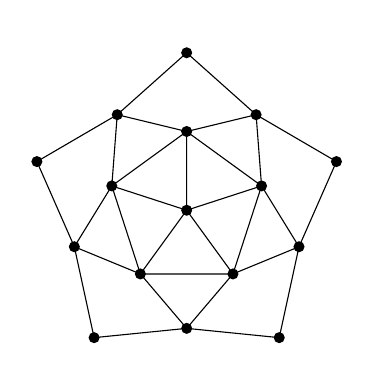
\begin{tikzpicture}

  \foreach \x in {0,...,4} {
  	\coordinate (a\x) at (18+\x*72:1cm);
  	\coordinate (b\x) at (18+\x*72:2cm);
  	\coordinate (c\x) at (54+\x*72:1.5cm);
  	\draw (0,0) -- (a\x) \v -- (c\x) \v -- (b\x) \v;
  }
  \draw (0,0) \v;
  \draw (a0) -- (a1) -- (a2) -- (a3) -- (a4) -- (a0);
  \draw (a0) -- (c4) (a1) -- (c0) (a2) -- (c1) (a3) -- (c2) (a4) -- (c3);
  \draw (b0) -- (c4) (b1) -- (c0) (b2) -- (c1) (b3) -- (c2) (b4)-- (c3);
  \end{tikzpicture}
  \end{center}

  \begin{parts}
  \part[4] Find a proper vertex coloring of the graph.  Color (or label) the graph above.

  \begin{solution}
  	You \emph{could} color every vertex a different color.  Or you could use as few as 4 colors: start with the center vertex and use three other colors for the adjacent vertices.  Continue working your way out.
  \end{solution}


  \part[3] Explain how you know the chromatic number of the graph cannot be more than 4.
  \begin{solution}
  The graph is planar, so the chromatic number is at most 4.  Alternatively, if you gave a 4-coloring above, you know the chromatic number must be 4 or less.
  \end{solution}

  \vfill
  \part[3] Explain how you know the chromatic number of the graph cannot be less than 4.
  \begin{solution}
  The vertex in the center and its 5 neighbors create a copy of $W_5$ (the 5-wheel), which requires 4 colors.  The cycle of 5 vertices requires 3 colors, and the center vertex must be a different color than those three.
  \end{solution}
  \vfill
  \end{parts}


\end{questions}
\end{document}
